\documentclass[a4paper,12pt]{article}
\usepackage{float}
\usepackage{hyperref}
\usepackage{graphicx}

\title{Final report}
\author{The Waypointers}

\begin{document}

%%%%%%%%%%%%%%%%%%%%%%%%%%%%%%%%%%%%%%%%%
% University Assignment Title Page 
% LaTeX Template
%
% This template has been downloaded from:
% http://www.LaTeXTemplates.com
%
% Original author:
% WikiBooks (http://en.wikibooks.org/wiki/LaTeX/Title_Creation)
%
% License:
% CC BY-NC-SA 3.0 (http://creativecommons.org/licenses/by-nc-sa/3.0/)i

\begin{titlepage}

\newcommand{\HRule}{\rule{\linewidth}{0.5mm}} % Defines a new command for the horizontal lines, change thickness here

\center % Center everything on the page
 
%----------------------------------------------------------------------------------------
%	HEADING SECTIONS
%----------------------------------------------------------------------------------------

\textsc{\LARGE King's College London}\\[1.5cm] % Name of your university/college
\textsc{\Large 7CCSMGPR Group Project}\\[0.5cm] % Major heading such as course name
%\textsc{\large Minor Heading}\\[0.5cm] % Minor heading such as course title

%----------------------------------------------------------------------------------------
%	TITLE SECTION
%----------------------------------------------------------------------------------------

\HRule \\[0.4cm]
{ \huge \bfseries Final project report}\\[0.4cm] % Title of your document
\HRule \\[1.5cm]
 
%----------------------------------------------------------------------------------------
%	AUTHOR SECTION
%----------------------------------------------------------------------------------------
\begin{flushleft}
{\Large \emph{Team:}\\
\textsc{The Waypointers}\\}
Haipei Liu\\
Karlo Santini\\
Michal Szewczak\\
Mengzhu Wang\\
Minghao Zhu\\[3cm]
\end{flushleft}
%----------------------------------------------------------------------------------------
%	DATE SECTION
%----------------------------------------------------------------------------------------

{\large \today}\\[3cm] % Date, change the \today to a set date if you want to be precise

%----------------------------------------------------------------------------------------
%	LOGO SECTION
%----------------------------------------------------------------------------------------

%\includegraphics{Logo}\\[1cm] % Include a department/university logo - this will require the graphicx package
 
%----------------------------------------------------------------------------------------

\vfill % Fill the rest of the page with whitespace

\end{titlepage}

%%%%%%%%%%%%%%%%%%%%%%%%%%%%%%%%%%%%%%%%%%

\tableofcontents

\section{Introduction}

\section{Review of related work}

\section{Requirements}
\subsection{Team work in requirement phase} The requirement analysis is a basic part of the whole project, which will influence every iterative process in the future development. So at the requirement analysis phase, we have twice meetings to discuss and define the requirements. We focused on The Task in Introductory Lecture, and extracted the list of features of the Traffic Simulation System. These features are presented in our initial report clearly.
\subsection{Functional requirements}  Based on these features, we got the functional requirements of the Traffic Simulation System. These requirements cover the vehicles, road network, traffic lights, the behaviors of drivers, simulation analysis and interaction between the user and the system. The following table will show the details of the functional requirements of the Traffic Simulation System.

\begin{table}[!htbp]
\centering
\label{versiontable}
\caption{Functional requirements}
\begin{tabular}{|p{1.5cm}|p{11cm}|}
\hline
ID & Functional Requirement\\
\hline
FR-1& The Traffic Simulation System should simulate different kinds of vehicles;\\
\hline
FR-2& The Traffic Simulation System should contain a road network, which contains straight roads with junctions;\\
\hline
FR-3& The Traffic Simulation System should allow user to set traffic lights in the junctions;\\
\hline
FR-4& The Traffic Simulation System should let vehicle enter the road network at a random entry, and leave at a random exit as well;\\
\hline
FR-5& The Traffic Simulation System should allow the user to add different kinds of vehicles into the road network;\\
\hline
FR-6& The Traffic Simulation System should simulate different behaviors of drivers, which includes reckless behavior, cautious behavior and normal behavior;\\
\hline
FR-7& The Traffic Simulation System should present real-time situation of the traffic, this should be a statistic result;\\
\hline
FR-8& The Traffic Simulation System should allow the user to control the simulation, including the starting or pausing, the time step, the speed of simulation, the states per second, the debug model and the interval of switching traffic lights.\\
\hline
\end{tabular}
\end{table}

\subsection{Quality requirement} To ensure the robustness of the system, we also determined the quality requirements of the system, which can improve the operation of the system. The details of the quality requirements of the Traffic Simulation System will be stated in the following table.

\begin{table}[!htbp]
\centering
\label{versiontable}
\caption{Functional Requirements}
\begin{tabular}{|p{1.5cm}|p{3cm}|p{8cm}|}
\hline
ID & Property & Functional Requirement\\
\hline
QR-1& Functionality&  The Traffic Simulation System should meet all the requirements from the users, and implement all the functions of the system;\\
\hline
QR-2& Maintainability& The Traffic Simulation System should be easy to maintain, the developer can modify the system and remove the defects very efficiently;\\
\hline
QR-3& Efficiency& The Traffic Simulation System should promptly respond to user's operations;\\
\hline
QR-4& Reliability& The Traffic Simulation System should ensure the low frequency of system crashes;\\
\hline
QR-5& Usability& The Traffic Simulation System should have a clear GUI interface that use can use it immediately and easily.\\
\hline\documentclass[a4paper,12pt]{article}
\usepackage{float}
\usepackage{longtable,tabu}
\usepackage{etoc}
\usepackage{listings}
\usepackage[usenames,dvipsnames]{color}
\usepackage[colorlinks=true,linkcolor=blue]{hyperref} 

\definecolor{codegreen}{rgb}{0,0.6,0}
\definecolor{codegray}{rgb}{0.5,0.5,0.5}
\definecolor{codepurple}{rgb}{0.58,0,0.82}
\definecolor{backcolour}{rgb}{0.95,0.95,0.92}

\lstdefinestyle{customasm}{
  backgroundcolor=\color{backcolour},   
  commentstyle=\color{codegreen},
  keywordstyle=\color{magenta},
  numberstyle=\tiny\color{codegray},
  stringstyle=\color{codepurple},
  basicstyle=\tiny\ttfamily,
  breakatwhitespace=false,         
  breaklines=true,                 
  captionpos=b,                    
  keepspaces=true,                 
  numbers=left,                    
  numbersep=5pt,                  
  showspaces=false,                
  showstringspaces=false,
  showtabs=false,                  
  tabsize=2,
  linewidth=14cm,
  language=Java
}
\lstdefinestyle{gitlog}{
  backgroundcolor=\color{backcolour},   
  commentstyle=\color{codegreen},
  keywordstyle=\color{magenta},
  numberstyle=\tiny\color{codegray},
  stringstyle=\color{codepurple},
  basicstyle=\tiny\ttfamily,
  breakatwhitespace=false,         
  breaklines=true,                 
  captionpos=b,                    
  keepspaces=true,                 
  numbers=left,                    
  numbersep=5pt,                  
  showspaces=false,                
  showstringspaces=false,
  showtabs=false,                  
  tabsize=2,
  linewidth=14cm,
} 

\title{Final report}
\author{The Waypointers}

\begin{document}

%%%%%%%%%%%%%%%%%%%%%%%%%%%%%%%%%%%%%%%%%
% University Assignment Title Page 
% LaTeX Template
%
% This template has been downloaded from:
% http://www.LaTeXTemplates.com
%
% Original author:
% WikiBooks (http://en.wikibooks.org/wiki/LaTeX/Title_Creation)
%
% License:
% CC BY-NC-SA 3.0 (http://creativecommons.org/licenses/by-nc-sa/3.0/)i

\begin{titlepage}

\newcommand{\HRule}{\rule{\linewidth}{0.5mm}} % Defines a new command for the horizontal lines, change thickness here

\center % Center everything on the page
 
%----------------------------------------------------------------------------------------
%	HEADING SECTIONS
%----------------------------------------------------------------------------------------

\textsc{\LARGE King's College London}\\[1.5cm] % Name of your university/college
\textsc{\Large 7CCSMGPR Group Project}\\[0.5cm] % Major heading such as course name
%\textsc{\large Minor Heading}\\[0.5cm] % Minor heading such as course title

%----------------------------------------------------------------------------------------
%	TITLE SECTION
%----------------------------------------------------------------------------------------

\HRule \\[0.4cm]
{ \huge \bfseries Final project report}\\[0.4cm] % Title of your document
\HRule \\[1.5cm]
 
%----------------------------------------------------------------------------------------
%	AUTHOR SECTION
%----------------------------------------------------------------------------------------
\begin{flushleft}
{\Large \emph{Team:}\\
\textsc{The Waypointers}\\}
Haipei Liu\\
Karlo Santini\\
Michal Szewczak\\
Mengzhu Wang\\
Minghao Zhu\\[3cm]
\end{flushleft}
%----------------------------------------------------------------------------------------
%	DATE SECTION
%----------------------------------------------------------------------------------------

{\large \today}\\[3cm] % Date, change the \today to a set date if you want to be precise

%----------------------------------------------------------------------------------------
%	LOGO SECTION
%----------------------------------------------------------------------------------------

%\includegraphics{Logo}\\[1cm] % Include a department/university logo - this will require the graphicx package
 
%----------------------------------------------------------------------------------------

\vfill % Fill the rest of the page with whitespace

\end{titlepage}

%%%%%%%%%%%%%%%%%%%%%%%%%%%%%%%%%%%%%%%%%%
\etocdepthtag.toc{mtchapter}
\etocsettagdepth{mtchapter}{subsection}
\etocsettagdepth{mtappendix}{section}
\tableofcontents

\newpage

\section{Introduction}

\section{Review of related work}

\section{Requirements}

\section{Design}

\section{Implementation}

\section{Teamwork}

\subsection{Tools and libraries used}

\subsubsection*{Tools and applications}

\begin{itemize}
	\item Git\footnote{\url{https://git-scm.com/}} - version control
	\item GitHub\footnote{\url{https://github.com/}} - Git repository management, task assignment, teamwork
	\item \LaTeX\footnote{\url{https://www.latex-project.org/}} - typesetting system, for creating documentation
	\item Gliffy\footnote{\url{https://www.gliffy.com/}} - a Chrome app for creating diagrams
	\item Apache Maven\footnote{\url{https://maven.apache.org/}} - a build tool for building the project easily and for dependency management
	\item Travis CI\footnote{\url{https://travis-ci.org/}} - a continuous integration tool that integrates into GitHub and builds every commit pushed to the repository (in our case - using Maven), also checking if the tests pass
	\item IntelliJ IDEA\footnote{\url{https://www.jetbrains.com/idea/}} - a cross-platform IDE for development in Java (and more). To minimize potential hassles with different development environments, we all agreed on using the same IDE.
\end{itemize}


A significant fact to note that is our team used all the major operating systems (Windows, OS X, Linux), so we focused on choosing cross-platform tools. The only troubles that arised from that were minor layout differences in the Swing GUI of our system.

\subsubsection*{Libraries}

\begin{itemize}
	\item JDK 1.8\footnote{\url{http://www.oracle.com/technetwork/java/javase/downloads/index.html}} - We had several reasons for choosing Java: \begin{itemize}
		\item Familiarity of team members with it
		\item Available on all platforms
		\item Good capabilities of cross-platform GUI
		\item Strong typing allowing for easier maintaining of code integrity
	\end{itemize}
	We chose version 8 because it introduces many much-needed improvements for the language like lambda functions or the Stream API.
	\item JUnit 4.12\footnote{\url{http://junit.org/junit4/}} - The ``de facto'' unit testing library for Java. Good integration with IntelliJ IDEA and Maven.
	\item FEST-Assert 2.0M5\footnote{\url{https://github.com/alexruiz/fest-assert-2.x}} - A library to make assertions in unit tests more readable and easier to compose.
	\item JGraphT 0.7.3 \footnote{\url{http://jgrapht.org/}} - A graph library to take advantage of graph representation of the road network, mainly pathfinding for vehicles.
	\item XStream 1.2.2 \footnote{\url{http://x-stream.github.io/}} - An XML serialization library to bring reading and writing XML road maps to life.
\end{itemize}



\section{Evaluation}

\section{Peer assessment}

\newpage
\appendix

\etocdepthtag.toc{mtappendix}
\etocsettagdepth{mtchapter}{none}
\etocsettagdepth{mtappendix}{subsection}
\tableofcontents‎‎

\section{Git log}

\lstinputlisting[style=gitlog]{gitlog.txt}

\section{Main source code}


\newpage
\subsection{Bootstrapper.java}
\lstinputlisting[style=customasm]{../../src/main/java/thewaypointers/trafficsimulator/Bootstrapper.java}
\newpage
\subsection{common/Direction.java}
\lstinputlisting[style=customasm]{../../src/main/java/thewaypointers/trafficsimulator/common/Direction.java}
\newpage
\subsection{common/ExitNodeDTO.java}
\lstinputlisting[style=customasm]{../../src/main/java/thewaypointers/trafficsimulator/common/ExitNodeDTO.java}
\newpage
\subsection{common/helpers/FirstVersionProvider.java}
\lstinputlisting[style=customasm]{../../src/main/java/thewaypointers/trafficsimulator/common/helpers/FirstVersionProvider.java}
\newpage
\subsection{common/helpers/InitialParameters.java}
\lstinputlisting[style=customasm]{../../src/main/java/thewaypointers/trafficsimulator/common/helpers/InitialParameters.java}
\newpage
\subsection{common/helpers/JunctionTestProvider.java}
\lstinputlisting[style=customasm]{../../src/main/java/thewaypointers/trafficsimulator/common/helpers/JunctionTestProvider.java}
\newpage
\subsection{common/helpers/RoadNetworkProvider.java}
\lstinputlisting[style=customasm]{../../src/main/java/thewaypointers/trafficsimulator/common/helpers/RoadNetworkProvider.java}
\newpage
\subsection{common/helpers/SimpleStateChangeListener.java}
\lstinputlisting[style=customasm]{../../src/main/java/thewaypointers/trafficsimulator/common/helpers/SimpleStateChangeListener.java}
\newpage
\subsection{common/ILocation.java}
\lstinputlisting[style=customasm]{../../src/main/java/thewaypointers/trafficsimulator/common/ILocation.java}
\newpage
\subsection{common/ISimulationInputListener.java}
\lstinputlisting[style=customasm]{../../src/main/java/thewaypointers/trafficsimulator/common/ISimulationInputListener.java}
\newpage
\subsection{common/IStateChangeListener.java}
\lstinputlisting[style=customasm]{../../src/main/java/thewaypointers/trafficsimulator/common/IStateChangeListener.java}
\newpage
\subsection{common/IStateProvider.java}
\lstinputlisting[style=customasm]{../../src/main/java/thewaypointers/trafficsimulator/common/IStateProvider.java}
\newpage
\subsection{common/JunctionDTO.java}
\lstinputlisting[style=customasm]{../../src/main/java/thewaypointers/trafficsimulator/common/JunctionDTO.java}
\newpage
\subsection{common/JunctionLocationDTO.java}
\lstinputlisting[style=customasm]{../../src/main/java/thewaypointers/trafficsimulator/common/JunctionLocationDTO.java}
\newpage
\subsection{common/JunctionMoveResult.java}
\lstinputlisting[style=customasm]{../../src/main/java/thewaypointers/trafficsimulator/common/JunctionMoveResult.java}
\newpage
\subsection{common/JunctionTrafficLightsDTO.java}
\lstinputlisting[style=customasm]{../../src/main/java/thewaypointers/trafficsimulator/common/JunctionTrafficLightsDTO.java}
\newpage
\subsection{common/Lane.java}
\lstinputlisting[style=customasm]{../../src/main/java/thewaypointers/trafficsimulator/common/Lane.java}
\newpage
\subsection{common/MapDTO.java}
\lstinputlisting[style=customasm]{../../src/main/java/thewaypointers/trafficsimulator/common/MapDTO.java}
\newpage
\subsection{common/NodeDTO.java}
\lstinputlisting[style=customasm]{../../src/main/java/thewaypointers/trafficsimulator/common/NodeDTO.java}
\newpage
\subsection{common/RoadDTO.java}
\lstinputlisting[style=customasm]{../../src/main/java/thewaypointers/trafficsimulator/common/RoadDTO.java}
\newpage
\subsection{common/RoadLocationDTO.java}
\lstinputlisting[style=customasm]{../../src/main/java/thewaypointers/trafficsimulator/common/RoadLocationDTO.java}
\newpage
\subsection{common/RoadTrafficLightsDTO.java}
\lstinputlisting[style=customasm]{../../src/main/java/thewaypointers/trafficsimulator/common/RoadTrafficLightsDTO.java}
\newpage
\subsection{common/SimulationInputListener.java}
\lstinputlisting[style=customasm]{../../src/main/java/thewaypointers/trafficsimulator/common/SimulationInputListener.java}
\newpage
\subsection{common/TrafficLightColor.java}
\lstinputlisting[style=customasm]{../../src/main/java/thewaypointers/trafficsimulator/common/TrafficLightColor.java}
\newpage
\subsection{common/TrafficLightDTO.java}
\lstinputlisting[style=customasm]{../../src/main/java/thewaypointers/trafficsimulator/common/TrafficLightDTO.java}
\newpage
\subsection{common/TrafficLightSystemDTO.java}
\lstinputlisting[style=customasm]{../../src/main/java/thewaypointers/trafficsimulator/common/TrafficLightSystemDTO.java}
\newpage
\subsection{common/VehicleDTO.java}
\lstinputlisting[style=customasm]{../../src/main/java/thewaypointers/trafficsimulator/common/VehicleDTO.java}
\newpage
\subsection{common/VehicleListDTO.java}
\lstinputlisting[style=customasm]{../../src/main/java/thewaypointers/trafficsimulator/common/VehicleListDTO.java}
\newpage
\subsection{common/VehicleType.java}
\lstinputlisting[style=customasm]{../../src/main/java/thewaypointers/trafficsimulator/common/VehicleType.java}
\newpage
\subsection{common/WorldStateDTO.java}
\lstinputlisting[style=customasm]{../../src/main/java/thewaypointers/trafficsimulator/common/WorldStateDTO.java}
\newpage
\subsection{FirstVersionStarter.java}
\lstinputlisting[style=customasm]{../../src/main/java/thewaypointers/trafficsimulator/FirstVersionStarter.java}
\newpage
\subsection{gui/ControlPanel.java}
\lstinputlisting[style=customasm]{../../src/main/java/thewaypointers/trafficsimulator/gui/ControlPanel.java}
\newpage
\subsection{gui/ControlPanelDocumentListener.java}
\lstinputlisting[style=customasm]{../../src/main/java/thewaypointers/trafficsimulator/gui/ControlPanelDocumentListener.java}
\newpage
\subsection{gui/GuiController.java}
\lstinputlisting[style=customasm]{../../src/main/java/thewaypointers/trafficsimulator/gui/GuiController.java}
\newpage
\subsection{gui/JumpOutDialog.java}
\lstinputlisting[style=customasm]{../../src/main/java/thewaypointers/trafficsimulator/gui/JumpOutDialog.java}
\newpage
\subsection{gui/MainFrame.java}
\lstinputlisting[style=customasm]{../../src/main/java/thewaypointers/trafficsimulator/gui/MainFrame.java}
\newpage
\subsection{gui/MainFrameEventHandle.java}
\lstinputlisting[style=customasm]{../../src/main/java/thewaypointers/trafficsimulator/gui/MainFrameEventHandle.java}
\newpage
\subsection{gui/MapContainerPanel.java}
\lstinputlisting[style=customasm]{../../src/main/java/thewaypointers/trafficsimulator/gui/MapContainerPanel.java}
\newpage
\subsection{gui/MapPanel.java}
\lstinputlisting[style=customasm]{../../src/main/java/thewaypointers/trafficsimulator/gui/MapPanel.java}
\newpage
\subsection{gui/PanelMouseAction.java}
\lstinputlisting[style=customasm]{../../src/main/java/thewaypointers/trafficsimulator/gui/PanelMouseAction.java}
\newpage
\subsection{gui/Statistics.java}
\lstinputlisting[style=customasm]{../../src/main/java/thewaypointers/trafficsimulator/gui/Statistics.java}
\newpage
\subsection{gui/StatisticsPanel.java}
\lstinputlisting[style=customasm]{../../src/main/java/thewaypointers/trafficsimulator/gui/StatisticsPanel.java}
\newpage
\subsection{JunctionLocationTestStarter.java}
\lstinputlisting[style=customasm]{../../src/main/java/thewaypointers/trafficsimulator/JunctionLocationTestStarter.java}
\newpage
\subsection{RoadNetworkStarter.java}
\lstinputlisting[style=customasm]{../../src/main/java/thewaypointers/trafficsimulator/RoadNetworkStarter.java}
\newpage
\subsection{simulation/enums/NodeType.java}
\lstinputlisting[style=customasm]{../../src/main/java/thewaypointers/trafficsimulator/simulation/enums/NodeType.java}
\newpage
\subsection{simulation/enums/VehicleType.java}
\lstinputlisting[style=customasm]{../../src/main/java/thewaypointers/trafficsimulator/simulation/enums/VehicleType.java}
\newpage
\subsection{simulation/factories/GraphFactory.java}
\lstinputlisting[style=customasm]{../../src/main/java/thewaypointers/trafficsimulator/simulation/factories/GraphFactory.java}
\newpage
\subsection{simulation/factories/MapWorldStateFactory.java}
\lstinputlisting[style=customasm]{../../src/main/java/thewaypointers/trafficsimulator/simulation/factories/MapWorldStateFactory.java}
\newpage
\subsection{simulation/factories/VehicleFactory.java}
\lstinputlisting[style=customasm]{../../src/main/java/thewaypointers/trafficsimulator/simulation/factories/VehicleFactory.java}
\newpage
\subsection{simulation/factories/xml/models/HandlerXML.java}
\lstinputlisting[style=customasm]{../../src/main/java/thewaypointers/trafficsimulator/simulation/factories/xml/models/HandlerXML.java}
\newpage
\subsection{simulation/factories/xml/models/JunctionXML.java}
\lstinputlisting[style=customasm]{../../src/main/java/thewaypointers/trafficsimulator/simulation/factories/xml/models/JunctionXML.java}
\newpage
\subsection{simulation/factories/xml/models/MapXML.java}
\lstinputlisting[style=customasm]{../../src/main/java/thewaypointers/trafficsimulator/simulation/factories/xml/models/MapXML.java}
\newpage
\subsection{simulation/factories/xml/models/RoadXML.java}
\lstinputlisting[style=customasm]{../../src/main/java/thewaypointers/trafficsimulator/simulation/factories/xml/models/RoadXML.java}
\newpage
\subsection{simulation/models/graph/helper/DistributedRandomNumberGenerator.java}
\lstinputlisting[style=customasm]{../../src/main/java/thewaypointers/trafficsimulator/simulation/models/graph/helper/DistributedRandomNumberGenerator.java}
\newpage
\subsection{simulation/models/graph/helper/Node.java}
\lstinputlisting[style=customasm]{../../src/main/java/thewaypointers/trafficsimulator/simulation/models/graph/helper/Node.java}
\newpage
\subsection{simulation/models/graph/helper/RoadEdge.java}
\lstinputlisting[style=customasm]{../../src/main/java/thewaypointers/trafficsimulator/simulation/models/graph/helper/RoadEdge.java}
\newpage
\subsection{simulation/models/graph/helper/TrafficLightNode.java}
\lstinputlisting[style=customasm]{../../src/main/java/thewaypointers/trafficsimulator/simulation/models/graph/helper/TrafficLightNode.java}
\newpage
\subsection{simulation/models/interfaces/IVehicle.java}
\lstinputlisting[style=customasm]{../../src/main/java/thewaypointers/trafficsimulator/simulation/models/interfaces/IVehicle.java}
\newpage
\subsection{simulation/models/managers/VehicleManager.java}
\lstinputlisting[style=customasm]{../../src/main/java/thewaypointers/trafficsimulator/simulation/models/managers/VehicleManager.java}
\newpage
\subsection{simulation/models/VehicleMap.java}
\lstinputlisting[style=customasm]{../../src/main/java/thewaypointers/trafficsimulator/simulation/models/VehicleMap.java}
\newpage
\subsection{simulation/models/vehicles/Car.java}
\lstinputlisting[style=customasm]{../../src/main/java/thewaypointers/trafficsimulator/simulation/models/vehicles/Car.java}
\newpage
\subsection{simulation/models/vehicles/EmergencyService.java}
\lstinputlisting[style=customasm]{../../src/main/java/thewaypointers/trafficsimulator/simulation/models/vehicles/EmergencyService.java}
\newpage
\subsection{simulation/Simulation.java}
\lstinputlisting[style=customasm]{../../src/main/java/thewaypointers/trafficsimulator/simulation/Simulation.java}
\newpage
\subsection{StateProviderController.java}
\lstinputlisting[style=customasm]{../../src/main/java/thewaypointers/trafficsimulator/StateProviderController.java}
\newpage
\subsection{TrafficSimulatorStarter.java}
\lstinputlisting[style=customasm]{../../src/main/java/thewaypointers/trafficsimulator/TrafficSimulatorStarter.java}
\newpage
\subsection{utils/Angle.java}
\lstinputlisting[style=customasm]{../../src/main/java/thewaypointers/trafficsimulator/utils/Angle.java}
\newpage
\subsection{utils/FloatPoint.java}
\lstinputlisting[style=customasm]{../../src/main/java/thewaypointers/trafficsimulator/utils/FloatPoint.java}
\newpage
\subsection{utils/Pair.java}
\lstinputlisting[style=customasm]{../../src/main/java/thewaypointers/trafficsimulator/utils/Pair.java}
\newpage
\subsection{utils/Rotation.java}
\lstinputlisting[style=customasm]{../../src/main/java/thewaypointers/trafficsimulator/utils/Rotation.java}
\newpage
\subsection{utils/SpeedConvert.java}
\lstinputlisting[style=customasm]{../../src/main/java/thewaypointers/trafficsimulator/utils/SpeedConvert.java}
\newpage
\subsection{utils/VehicleSpawnRatio.java}
\lstinputlisting[style=customasm]{../../src/main/java/thewaypointers/trafficsimulator/utils/VehicleSpawnRatio.java}


\section{Test source code}


\newpage
\subsection{tests/common/helpers/FirstVersionProviderTest.java}
\lstinputlisting[style=customasm]{../../src/test/java/thewaypointers/trafficsimulator/tests/common/helpers/FirstVersionProviderTest.java}
\newpage
\subsection{tests/common/JunctionLocationDTOTest.java}
\lstinputlisting[style=customasm]{../../src/test/java/thewaypointers/trafficsimulator/tests/common/JunctionLocationDTOTest.java}
\newpage
\subsection{tests/common/MapDTOTest.java}
\lstinputlisting[style=customasm]{../../src/test/java/thewaypointers/trafficsimulator/tests/common/MapDTOTest.java}
\newpage
\subsection{tests/FirstVersionStarterTest.java}
\lstinputlisting[style=customasm]{../../src/test/java/thewaypointers/trafficsimulator/tests/FirstVersionStarterTest.java}
\newpage
\subsection{tests/gui/GuiControllerTest.java}
\lstinputlisting[style=customasm]{../../src/test/java/thewaypointers/trafficsimulator/tests/gui/GuiControllerTest.java}
\newpage
\subsection{tests/JunctionLocationTestStarterTest.java}
\lstinputlisting[style=customasm]{../../src/test/java/thewaypointers/trafficsimulator/tests/JunctionLocationTestStarterTest.java}
\newpage
\subsection{tests/RoadNetworkStarterTest.java}
\lstinputlisting[style=customasm]{../../src/test/java/thewaypointers/trafficsimulator/tests/RoadNetworkStarterTest.java}
\newpage
\subsection{tests/TrafficSimulatorStarterTest.java}
\lstinputlisting[style=customasm]{../../src/test/java/thewaypointers/trafficsimulator/tests/TrafficSimulatorStarterTest.java}
\newpage
\subsection{tests/utils/FloatPointTest.java}
\lstinputlisting[style=customasm]{../../src/test/java/thewaypointers/trafficsimulator/tests/utils/FloatPointTest.java}
\newpage
\subsection{utils/AngleTest.java}
\lstinputlisting[style=customasm]{../../src/test/java/thewaypointers/trafficsimulator/utils/AngleTest.java}


\end{document}


\end{tabular}
\end{table}

\section{Design}

\section{Implementation}
\subsection{Interaction between the user and the system}
\subsubsection{Description} The majority of interactions between the user and the system come from the Control Panel. The user can control the system through the components in the Control Panel, and the relevant corresponding will be showed in the specific area. The Control Panel can be separated into three parts, they are Simulation Controller, Vehicles Controller and the Traffic Lights Controller. Though Simulation Controller part, the user can control the starting or pausing of the simulation, the clear of the whole simulation, the time step of the simulation, the speed of the timer, the states per second of the simulation, and the display of the debug mode. As to the Vehicles Controller, the user can set the percentage of the different kinds of vehicles, and the behaviors of the drivers. In addition, the interval of switching the traffic lights can be set by the user through the Traffic Lights Controller.
The other interactions happen on the Map Panel. First of all, the user can drag and move the map to see more details of the simulation. Because the size of the map is bigger than the size of the Map Panel, we use this solution to help the user to see the complete map information. Then the user can set or remove the traffic lights just by clicking on the specific junction showed on the map.

\subsubsection{Design and implementation}
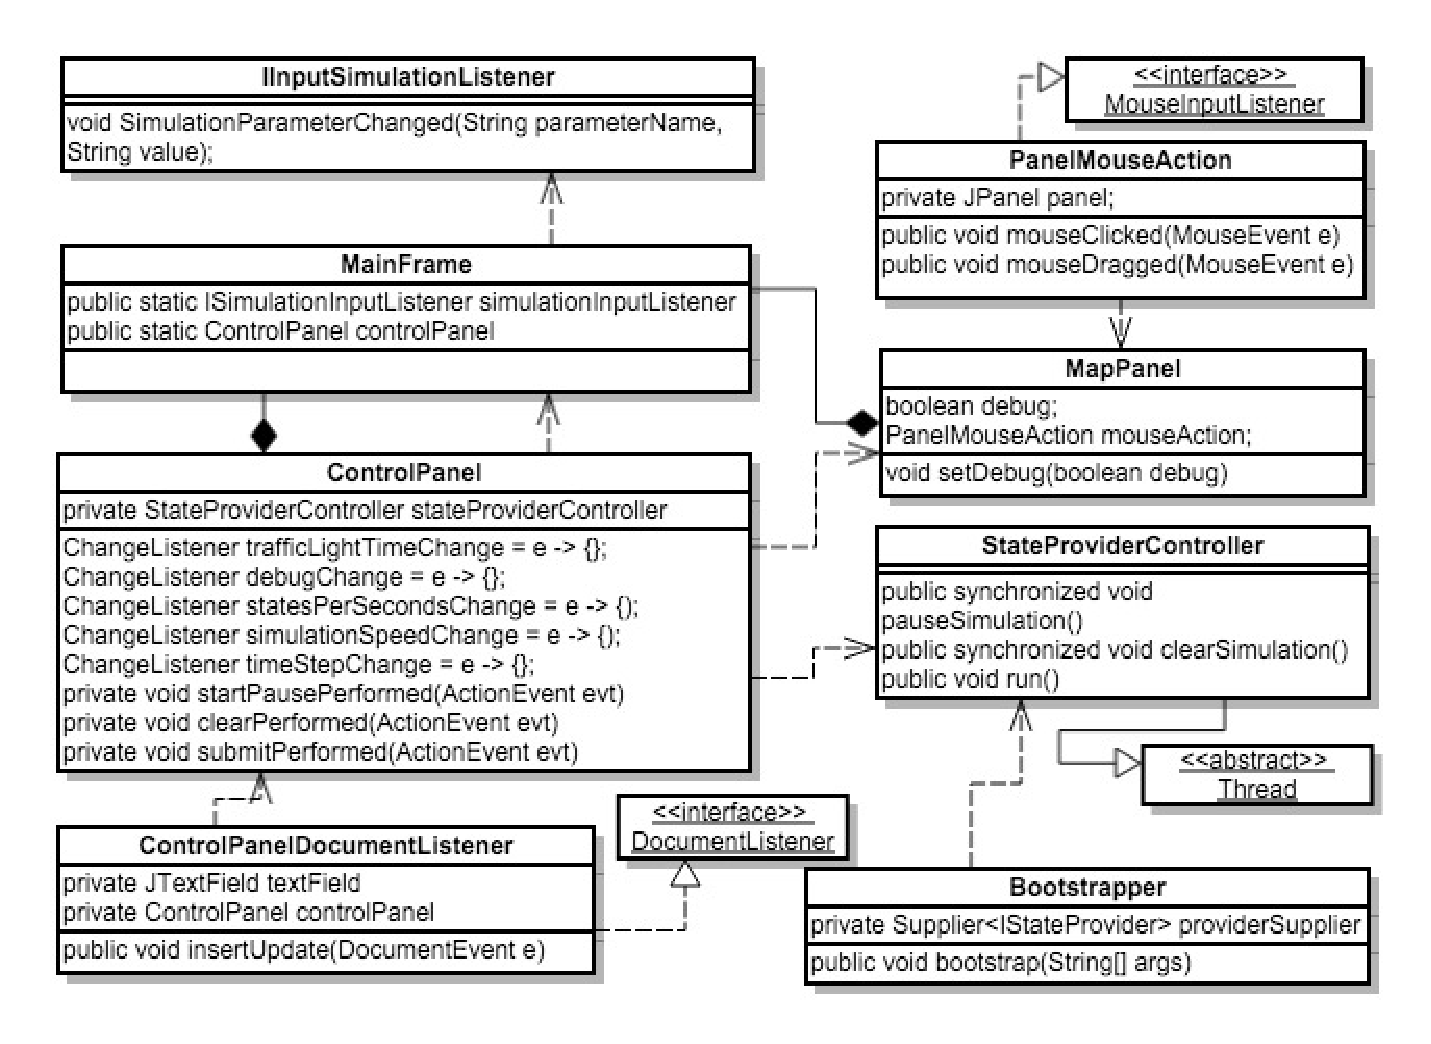
\includegraphics[width=12.5cm]{class.eps}
\paragraph{Class PanelMouseAction} implements MouseInputListener, which is added on the Map Panel. The main task for this class is processing the requests from the Mouse operation in the Map Panel. The first operation is dragging the map. It is easy to implement the function of dragging the panel, however, it will get more complex if we take the range into consider. The map in our system is a rectangle that has limited length and height. So the range of dragging should be the minimum length and width to maximum length and width. The second one is set or remove the traffic lights. In order to ensure the operability, the selectable range should be enlarged to the whole junction. After clicking the junction, the relevant parameters will be sent back to the "common" package.
\paragraph{Class ControlPanel} extends JPanel, which is added on the Main Frame. It is responsible for most of the interaction works. It uses the static parameter simulationListener in MainFrame to transfer inputs from the user to the server end mostly. While for the setting of debug mode, it transfers the Boolean parameter to the MapPanel directly. In addition, it should do the necessary checking of inputs before passing the values to the server side. For the invalid inputs, it will generate a JDialog object to prompt the user to make the appropriate changes. As to the control of starting or pausing, clearing of the simulation. It will use stateProviderController to control the main thread of the system.
\paragraph{Class ControlPanelDocumentListnener} implements DocumentListener, which is added to the text fields in Control Panel. It is used to check the validity of inputs. If the input is invalid, a JDialog that has related information will be generated.
\paragraph{Class StateProviderController} extends Thread, which is the main thread of the simulation. The thread is generated by the Bootstrapper class, and it keeps sleep state until the user starts the simulation. The Boolean parameter isSleep controlled the starting and pausing of the simulation. When the user chooses to clear the simulation, a new StateProvider will be passed to the simulation.
\paragraph{Class Bootstrapper} is generated by the main starter of the system. It is used to create the main thread StateProviderController and start it. It also generates the Main Frame and set relevant parameters of the simulation.


\subsubsection{Detailed description of the main function}

\paragraph{ChangeListener trafficLightTimeChange} This function is used to pass the value of the interval of switching traffic lights to the package "common". The input value that is set by the user will be passed through the function SimulationParameterChanged() of simulationInputListener in MainFrame.
\paragraph{ChangeListener debugChange} This function is used to pass a Boolean value to MapPanel to control whether display debug mode. 
\paragraph{ChangeListener statesPerSecondsChange} This function is used to pass the value of the states per seconds of the simulation to the package "common". The input value that is set by the user will be passed through the function SimulationParameterChanged() of simulationInputListener in MainFrame.
\paragraph{ChangeListener simulationSpeedChange} This function is used to pass the value of the speed of timer to the package "common". The input value that is set by the user will be passed through the function SimulationParameterChanged() of simulationInputListener in MainFrame.
\paragraph{ChangeListener timeStepChange}This function is used to pass the value of the time step of simulation to the package "common". The input value that is set by the user will be passed through the function SimulationParameterChanged() of simulationInputListener in MainFrame.
\paragraph{startPausePerformed(ActionEvent evt)} This function is used to control the main thread of the simulation. When the user presses the start button, the simulation will get start and the button will change to pause. When the user presses the pause button, the simulation will pause and the button change to start.
\paragraph{clearPerformed(ActionEvent evt)} This function is used to end the main thread of the simulation. When the user presses the clear button, the simulation will stop immediately.
\paragraph{submitPerformed(ActionEvent evt)} This function is used to pass the percentages of different kinds of vehicles to the package ?common?. The input value that is set by the user will be passed through the function SimulationParameterChanged() of simulationInputListener in MainFrame. At the same time, the validity of the input will be checked in this method.

\paragraph{mouseClicked(ActionEvent evt)} This function allows the user to set traffic lights at junctions. When the user clicks on a junction showed on the map, it will set or remove the traffic lights on this junction. The chosen traffic light will be passed through the function SimulationParameterChanged() of simulationInputListener in MainFrame. 
\paragraph{mouseDragged(ActionEvent evt)} This function allows the user to drag map inside of the MapPanel and see more details of the simulation. When the user drags the map, the system will check whether the map is in the visible field. If the new location out of the range, the map will be set at the border of the MapPanel.

\paragraph{pauseSimulation()} This function is used to control the main thread of the simulation. It will be invoked when the user presses the start/pause button. If the operation is  "start" then the thread will run as normal, while if the operation is "pause" then the thread will sleep until the user starts the simulation again.
\paragraph{clearSimulation()} This function is used to end the main thread of the simulation. It will be invoked when the user presses the clear button. The thread will stop immediately and generate a new thread of the simulation.
\paragraph{run()}This reconstructed function is used to execute the main thread of the simulation. It will be invoked when the system starts up.

\paragraph{insertUpdate(DocumentEvent e)} This reconstructed function is used to check the validity of the inputs. It will be invoked when the text field has new inputs.  If the input is invalid, a JDialog will pop up to display related information.

\paragraph{bootstrap(String[] args)} This function is used to generate a new thread StateProviderController and start the thread. It also generates the new MainFrame with relevant parameters of simulation controlling. This function is invoked by the main starter of the system.

\section{Teamwork}

\subsection{Tools and libraries used}

\subsubsection*{Tools and applications}

\begin{itemize}
	\item Git\footnote{\url{https://git-scm.com/}} - version control
	\item GitHub\footnote{\url{https://github.com/}} - Git repository management, task assignment, teamwork
	\item \LaTeX\footnote{\url{https://www.latex-project.org/}} - typesetting system, for creating documentation
	\item Gliffy\footnote{\url{https://www.gliffy.com/}} - a Chrome app for creating diagrams
	\item Apache Maven\footnote{\url{https://maven.apache.org/}} - a build tool for building the project easily and for dependency management
	\item Travis CI\footnote{\url{https://travis-ci.org/}} - a continuous integration tool that integrates into GitHub and builds every commit pushed to the repository (in our case - using Maven), also checking if the tests pass
	\item IntelliJ IDEA\footnote{\url{https://www.jetbrains.com/idea/}} - a cross-platform IDE for development in Java (and more). To minimize potential hassles with different development environments, we all agreed on using the same IDE.
\end{itemize}


A significant fact to note that is our team used all the major operating systems (Windows, OS X, Linux), so we focused on choosing cross-platform tools. The only troubles that arised from that were minor layout differences in the Swing GUI of our system.

\subsubsection*{Libraries}

\begin{itemize}
	\item JDK 1.8\footnote{\url{http://www.oracle.com/technetwork/java/javase/downloads/index.html}} - We had several reasons for choosing Java: \begin{itemize}
		\item Familiarity of team members with it
		\item Available on all platforms
		\item Good capabilities of cross-platform GUI
		\item Strong typing allowing for easier maintaining of code integrity
	\end{itemize}
	We chose version 8 because it introduces many much-needed improvements for the language like lambda functions or the Stream API.
	\item JUnit 4.12\footnote{\url{http://junit.org/junit4/}} - The ``de facto'' unit testing library for Java. Good integration with IntelliJ IDEA and Maven.
	\item FEST-Assert 2.0M5\footnote{\url{https://github.com/alexruiz/fest-assert-2.x}} - A library to make assertions in unit tests more readable and easier to compose.
	\item JGraphT 0.7.3 \footnote{\url{http://jgrapht.org/}} - A graph library to take advantage of graph representation of the road network, mainly pathfinding for vehicles.
	\item XStream 1.2.2 \footnote{\url{http://x-stream.github.io/}} - An XML serialization library to bring reading and writing XML road maps to life.
\end{itemize}



\section{Evaluation}

\section{Peer assessment}

\end{document}
